% Slide aspect ratio, theme and color theme
\documentclass[aspectratio=169]{beamer}
\usetheme{metropolis}
\usecolortheme[snowy]{owl}

% Modern font setup
\usepackage{fontspec}
\usepackage{unicode-math}

% Font selection
\setmainfont{Fira Sans}
\setsansfont{Fira Sans}
\setmonofont[
  UprightFont   = *,
  BoldFont      = *-Bold,
  ItalicFont    = *,    % <-- force regular to be used as “italic”
  BoldItalicFont= *-Bold        % <-- or omit if you don’t need Bold Italic
]{Fira Code}
% \setmathfont{Fira Math}

% Language and layout
\usepackage[utf8]{inputenc}
\usepackage[brazil]{babel}

% Good to keep
\usepackage{amsmath}
\usepackage{graphicx}
\usepackage{url}
\usepackage{xcolor}
\usepackage{xstring}
\usepackage{outlines}

% Bibliography
\usepackage[backend=biber,style=authoryear]{biblatex}
\addbibresource{references.bib}
\renewcommand*{\nameyeardelim}{\addcomma\space}
\renewcommand*{\bibfont}{\color{black}\small}
\setbeamercolor{bibliography item}{fg=black}
\setbeamercolor{bibliography entry author}{fg=black}
\setbeamercolor{bibliography entry title}{fg=black}
\setbeamercolor{bibliography entry location}{fg=black}
\setbeamercolor{bibliography entry note}{fg=black}

% Wrapper for figures
\newcommand{\insertfigure}[3]{
  \StrBehind{#1}{/}[\FileWithExt]
  \StrBefore{\FileWithExt}{.}[\FileName]
  \begin{figure}[h!]
    \vspace{0.25cm}
    \centering
    \includegraphics[width=#3\linewidth]{#1}
    \caption{#2}
    \label{fig:\FileName}
  \end{figure}
}

% Shortcuts for MDP variables
\newcommand{\St}{\mathbf{S}}
\newcommand{\A}{\mathbf{A}}
\newcommand{\R}{\mathbf{R}}
\newcommand{\Ptr}{\mathbf{P}}
\newcommand{\Obs}{\mathbf{O}}

% END PREAMBLE

\title{Sintetizando episódios de treino via abstração de jogos em Aprendizado por Reforço}
\author{Marcelo Augusto Salomão Ganem}
\institute{Departamento de Ciência da Computação \\ Universidade Federal de Minas Gerais}
\date{\today}
\begin{document}

\makeatletter

\begin{frame}
\titlepage
\end{frame}

\begin{frame}{Resumo}
    Este trabalho pretende verificar a efetividade da \textbf{sintetização de episódios utilizando modelagens abstrativas} dos jogos Blackjack e \textit{Settlers of Catan} seguindo a sintaxe \textit{Machinations} \parencite{machinations} no treino de agentes de aprendizado por reforço. 

    As políticas obtidas serão analisadas contra \textit{baselines} em implementações concretas dos jogos modelados para verificar a efetividade das intervenções propostas na velocidade e qualidade do aprendizado.

\end{frame}

% \begin{frame}{Outline}
% \tableofcontents
% \end{frame}


\section{Contexto}

\begin{frame}{Diagramas \textit{Machinations}}
        \begin{columns}
            \begin{column}{0.5\textwidth}
                \vspace{0.25cm}

                A sintaxe Machinations introduz regras para a representação de jogos a uma variedade de níveis de abstração.
                \vspace{0.25cm}

                O modelo representa um jogo como um diagrama de nós e conexões de diversos tipos entre eles. Assim, o estado do jogo é a distribuição de \textbf{recursos} entre os nós.
            \end{column}
            \begin{column}{0.5\textwidth}
                \insertfigure
                    {figures/catan.png}
                    {Uma representação do jogo \textit{Settlers of Catan} sob a sintaxe de Machinations \parencite{machinations}}
                    {0.8}
            \end{column}
        \end{columns}
    
\end{frame}

\begin{frame}{Diagramas \textit{Machinations}}
    \begin{figure}[h!]
        \begin{columns}
            \begin{column}{0.6\textwidth}
                \vspace{0.5cm}
                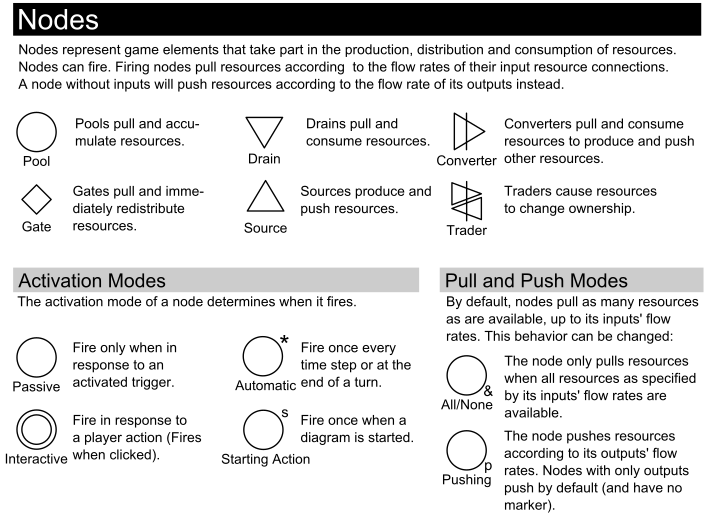
\includegraphics[width=1.0\linewidth]{figures/nodes.png}
            \end{column}
            \begin{column}{0.4\textwidth}
                \caption{Trecho do Apêndice A de \textit{Engineering Emergence} \parencite{machinations} descrevendo elementos básicos dos diagramas}
            \end{column}
        \end{columns}
        \label{fig:nodes}
    \end{figure}
\end{frame}

\begin{frame}{Diagramas \textit{Machinations}}
    \begin{columns}
        \begin{column}{0.5\textwidth}
	    A proposta da sintaxe é capturar e evidenciar relações na "economia interna" \ \parencite{machinations} do jogo a partir de suas regras. 

	    % A partir da definição dos elementos que compõem um diagrama e das conexões entre eles, é possível representar um único jogo de múltiplas maneiras.
        \end{column}
        \begin{column}{0.5\textwidth}
            \insertfigure
              {figures/monopoly.png}
              {\textit{Monopoly} (\citeyear{monopoly}) representado como um diagrama \textit{Machinations} \parencite{machinations}.}
              {1.0}
        \end{column}
    \end{columns}
\end{frame}


\begin{frame}{Diagramas \textit{Machinations}}
    As regras definidas por \citeauthor{machinations} não são formais o suficiente para permitir implementação direta\footnote{À época da publicação, existia uma simulação dinâmica disponível para o público -- hoje o serviço é prestado como B2B pela empresa Machinations, sediada na Holanda}. Assim, parte desse trabalho é transcrever a definição descritiva para uma definição formal.
\end{frame}

\section{Objetivos}

\begin{frame}{Objetivos}
    Utilizando diagramas Machinations como base, pretende-se \textbf{acelerar o treino de agentes de aprendizado por reforço via episódios sintetizados} como objetivo geral. Entendendo os diagramas como abstrações de problemas de aprendizado por reforço, o trabalho endereça especificamente as seguintes perguntas de pesquisa:
    \begin{outline}
        \1 Agentes treinados \textit{somente} na abstração produzem políticas coerentes no problema real?
        \1 É possível extrair representações úteis explorando a abstração?
    \end{outline}
\end{frame}

\section{Trabalhos Relacionados}
\begin{frame}{Curriculum Learning}
    O trabalho de \citeauthor{curriculum-learning} (\citeyear{curriculum-learning}) fundamenta a ideia de aprendizado por tarefas sucessivas de complexidade crescente. Especificamente, dada a coerência entre os ambientes e tarefas apresentadas, \citeauthor{curriculum-learning} provam que essa técnica \textbf{acelera a convergência} no treino.

    A princípio, entendemos o aprendizado no ambiente modelado em Machinations como a tarefa inicial (de otimização mais genérica), e o aprendizado no ambiente completo como a segunda e última tarefa do currículo (refinando a otimização anterior).
\end{frame}
\begin{frame}{Near Optimal Behavior via Approximate State Abstraction}
    \citeauthor{approximate-state-abstraction} (\citeyear{approximate-state-abstraction}) concluem que a qualidade de comportamentos derivados de abstrações aproximadas -- isto é, MDPs simplificados -- é preservada contra o caso base desde que a abstração seja suficientemente representativa\footnote{Conforme critérios específicos, não arbitrários.}.

    Além disso, o trabalho explicita vantagens de representações abstrativas aproximadas\footnote{Em distinção a aproximações de estado baseadas em regras e equivalência exata} em termos de tratabilidade (de espaços de estado), incorporação de planejamento e flexibilidade do grau de agrupamento de estados.
\end{frame}


\section{Metodologia}

\begin{frame}{Metodologia}
    \begin{outline}[enumerate]
	\1 Definição de diagramas Machinations como MDPs
	\1 Implementação do MDP e ambientes de avaliação\footnote{Implementação que clona o jogo e oferece uma API} para:
            \2 Blackjack
            \2 Settlers of Catan
	\1 Auxiliar o treino de agentes de RL com o MDP abstrativo
	\1 Comparar contra modelos idênticos treinados sem o MDP abstrativo em função de:
	    \2 Velocidade de convergência
	    \2 Qualidade da política obtida
    \end{outline}
\end{frame}

\begin{frame}{Formalizando diagramas \textit{Machinations}}
    "\textbf{Nós} são representados como vértices $v \in V$, seu estado $x_{v,r}: V \times R \rightarrow \mathbb{R}$ (o número de recursos do tipo $r$ no nó $v$) e a função $m_{v}: V \rightarrow \{0,1,2\}$ como o modo de ativação do nó entre passivo, automático ou interativo [...]"
\end{frame}

\begin{frame}{Formalizando diagramas \textit{Machinations}}

    \begin{columns}
        \begin{column}{0.4\textwidth}
            \vspace{0.75cm}

            \textit{"Triggers fire when all the inputs of its source node become satisfied: when each input passed the number of resources to the node as indicated by its flow rate"}
        \end{column}
        \begin{column}{0.1\textwidth}
            \begin{center}
                $\rightarrow$
            \end{center}
        \end{column}
        \begin{column}{0.4\textwidth}
            \vspace{0.75cm}
            \begin{align*}
                &\{v: (u \rightarrow v) \in E^G\ | \\\ &\Big(\prod_{e \in E^R | e = (* \rightarrow u)}{\Delta e(t-1) = T_e \Big)} = 1 \}\\
            \end{align*}
        \end{column}
    \end{columns}
\end{frame}

\begin{frame}{Definindo o POMDP}
    \begin{columns}
	\begin{column}{0.5\textwidth}
	    Definimos o espaço de estados do MDP como $\St = \{x_v: v \in V\} \times \{T_e: e \in R \}$ -- isto é, o número de recursos de cada tipo em cada vértice e a taxa de cada uma das conexões de recursos.

	    \vspace{0.25cm}

	    Ações são definidas como o conjunto potência dos vértices interativos: $\A = \mathcal{P}(\{ v \in V^A \})$
	\end{column}
	\begin{column}{0.5\textwidth}
	    \insertfigure
		{figures/risk.png}
        {\textit{Loop} central do jogo \textit{Risk} \parencite{machinations}}
		{1.0}
	\end{column}
    \end{columns}
\end{frame}

\begin{frame}{Definindo o POMDP}

    \vspace{0.25cm}

    Definimos pesos $\omega$ e $\rho$ para cada nó e conexão de recursos, respectivamente. Seguindo o princípio de \textit{potential-based shaping} \parencite{potential-rl}, temos:
    $$
	\Phi(s) = \sum_{v\in V^{\Phi}}\sum_{r \in R^{\Phi}}\omega_{v,r}\,x_{v,r}+\sum_{e\in E^{R^{\Phi}}}\rho_{e}\,T_{e}
    $$
    $$
    \R(s,a,s') = \Phi(s') \;-\; \Phi(s)
    $$

    \vspace{0.25cm}

    A dinâmica do MDP, por fim, é definida pela simulação do diagrama Machinations.

    % Assim, para cada especificação de diagrama Machinations, pode-se definir também os critérios específicos de recompensa conforme cada um dos nós. Ainda, a definição da função de potencial $\Phi$ facilita a extensão do esquema de recompensas conforme novos critérios.

\end{frame}

\begin{frame}{Interface comum}
    \begin{columns}
	\begin{column}{0.5\textwidth}
        O agente efetivamente interage com POMDPs de dinâmicas distintas por meio de uma mesma interface. Assim, podemos verificar a qualidade das políticas obtidas a partir da abstração diretamente na sua contraparte mais complexa (o jogo).

	\end{column}
	\begin{column}{0.5\textwidth}
	    \insertfigure
		{figures/arquitetura.png}
		{Sob a perspectiva do agente, a dinâmica do MDP é indistinta entre a simulação do diagrama e do jogo.}
		{0.8}
	\end{column}
    \end{columns}
\end{frame}

\begin{frame}{Implementação}
    \begin{columns}
	\begin{column}{0.6\textwidth}
	    \insertfigure
		{figures/implementacao.png}
		{Arquitetura da implementação do projeto}
		{1.0}
	\end{column}
	\begin{column}{0.4\textwidth}
	    \begin{outline}
		 \1 Ambiente Gymnasium
                \2 Simulação do Jogo
                \2 Simulação do Diagrama
		 \1 Algoritmos de RL
                \2 Q-Learning
                \2 PPO
		 \1 Visualizações com Manim
                \2 Sequências de estados do diagrama e do agente
	    \end{outline}
	\end{column}
    \end{columns}
\end{frame}

\begin{frame}{Plano de experimentos}
    \begin{outline}
	\1 Testes de sanidade: Blackjack + Q-Learning
	    \2 Garantir convergência no caso simples
	\vspace{0.25cm}
	\1 Aprendizado profundo: \textit{Settlers of Catan} + PPO
	    \2 Responder a padrões no diagrama % Caso do monopoly
	    \2 Lidar com espaços de estado maiores % Muitos nós, tipos de recurso e conexões
    \end{outline}
\end{frame}

\begin{frame}[shrink=5]
    \vspace{0.75cm}
    \printbibliography
\end{frame}


\end{document}

